\documentclass[12pt]{article}
\usepackage[a4paper, margin=1in]{geometry}
\usepackage[utf8]{inputenc}
\usepackage{titlesec}
\usepackage{enumitem}
\usepackage{graphicx}
\usepackage{titling}
\usepackage{longtable}
\usepackage{booktabs}
\usepackage[hidelinks]{hyperref}
\usepackage{fancyhdr}
\usepackage{setspace}
\usepackage{caption}
\usepackage{cite}
\usepackage{amsmath}
\usepackage{float}
\usepackage{tikz}
\usetikzlibrary{positioning}
\pagestyle{fancy}
\fancyhf{}
\rhead{CSE 816: DevOps}
\lhead{Final Project}
\rfoot{\thepage}
\titleformat{\section}{\normalfont\Large\bfseries}{\thesection}{1em}{}
\titleformat{\subsection}{\normalfont\large\bfseries}{\thesubsection}{1em}{}
\setstretch{1.2}
\pretitle{%
  \begin{center}
    
\includegraphics[width=0.25\textwidth]{logo.jpeg}\\[1em]  % Logo
    \large CSE 816 : Software Production Engineering\\
    \large Final Project \\[2em]  % Some spacing before the main title
    \LARGE
}
\title{\textbf{Automated creation and deployment of a Mail System}}
\posttitle{\end{center}}
\author{
    AMEDEKA Tsevi Christian: MS2024502
    \\[2\baselineskip]
    \textbf{Instructor: Prof B. Thangaraju}
}
\date{May 2025}

\begin{document}
\maketitle
\newpage
%\tableofcontents
\listoffigures
\newpage

\section{Introduction}

Email services are essential in personal, academic, and enterprise communication. Hosting a self-managed email server provides full control over data, privacy, and server configurations. The goal of this project is to develop and deploy a secure, scalable, and automated mail server infrastructure using open-source technologies and DevOps practices. The solution includes Postfix as the Mail Transfer Agent (MTA), Dovecot as the Mail Delivery Agent (MDA), Roundcube as the Mail User Agent (MUA), MySQL for database support, and a PHP-based web administration tool. The deployment and configuration process is fully automated using Docker, Docker Compose, Ansible, and Jenkins.

\section{System Architecture. }
The architecture consists of several modular components :
\begin{itemize}
    \item Postfix as MTA (Mail Transfer Agent). So Postfix is configured to send and receive email messages using the SMTP protocol. It handles mail routing and relaying, including authentication and TLS encryption for secure delivery.

    \item Dovecot as MDA (Mail Delivery Agent).  Dovecot delivers mail to users' mailboxes and allows them to retrieve mail using IMAP and POP3. It also provides authentication services for Postfix, including integration with MySQL for virtual users.

    \item MySQL database : The database stores virtual user information, including email addresses, hashed passwords, and domain associations. It also provides authentication support for both Postfix and Dovecot.

    \item A web administration tool: A lightweight web interface built with PHP allows administrators to create, modify, and delete user accounts. It communicates directly with the MySQL database.

\end{itemize}

All components are containerized using Docker and orchestrated using Docker Compose. Each service runs in a separate container with its own configuration, network, and volume bindings.

\section{System Diagram}
Next, we have a picture of the system diagram in a starred topology network
 
\begin{center}
    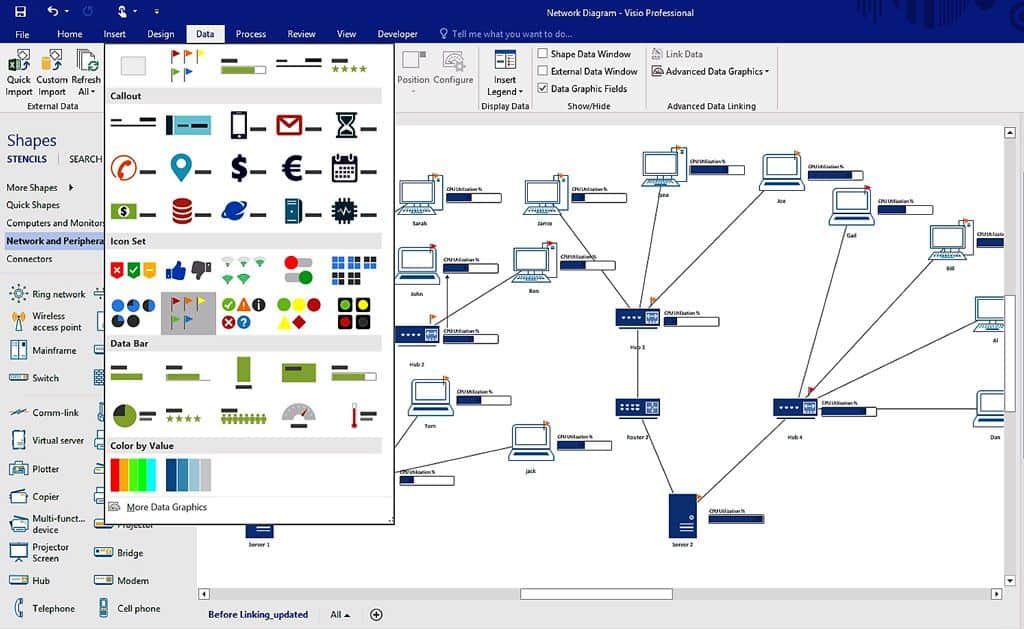
\includegraphics[width=0.9\textwidth]{diagram.png}
    \captionof{figure}{System Architecture Diagram} \label{diagram.png}
\end{center}

\section{Devops tool chain de deployment strategy}
To Streamline, the configuration, the continous delivery as well as the deployment, we used the following DevOps tools: 
\begin{itemize}
    \item Git: we used it to control the different versions of the system, created Github hook to trigger automatically the build of the project everytime we push code to Github.
    \item Docker: We used docker containers to encapsulate each service (Postfix, Dovecot, Roundube, Mysql and the web admin tool). We built the containers using Dockerfiles, ubuntu as base image and we included our own configuration files.
    \item Docker Compose: We used docker compose to define the services, their interdependencies, the network as well as volumes. This allow a seamless startup using a single command.
    \item Ansible: We automated the task such as the deployment of the system as well as some configurations
    \item Jenkins: We used jenkins to create a CI/CD pipeline that pulls the code from Github. I this pipeline, we built docker images, pushed them to docker hub, run the containers and deploy them. To do so, we creaded a Jenkinsfile which defined stages including the checkout, the build, the test and the deployment
\end{itemize}
Here is a visual of the DevOps tool chain workflow used 
\begin{figure}[H]
\centering
\begin{tikzpicture}[node distance=1cm and 1cm]

% Git
\node[inner sep=0pt] (git) 
  {
\includegraphics[width=2.5cm]{git.jpg}};
\node[below=2pt of git] {\small Git};

% Docker
\node[inner sep=0pt, right=of git] (docker)
  {
\includegraphics[width=2.5cm]{docker.jpg}};
\node[below=2pt of docker] {\small Docker};

% Compose
\node[inner sep=0pt, right=of docker] (compose)
  {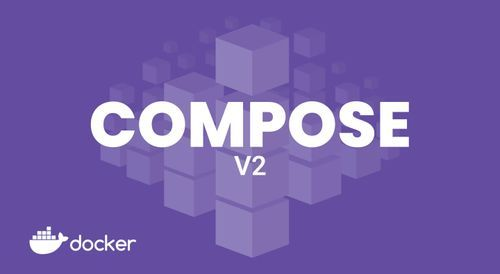
\includegraphics[width=2.5cm]{compose.jpg}};
\node[below=2pt of compose] {\small Docker Compose};

% Ansible
\node[inner sep=0pt, right=of compose] (ansible)
  {
\includegraphics[width=2.5cm]{ansible.jpg}};
\node[below=2pt of ansible] {\small Ansible};

% Jenkins
\node[inner sep=0pt, right=of ansible] (jenkins)
  {
\includegraphics[width=2.5cm]{jenkins.jpg}};
\node[below=2pt of jenkins] {\small Jenkins};

% Arrows
\draw[->, thick] (git.east) -- (docker.west);
\draw[->, thick] (docker.east) -- (compose.west);
\draw[->, thick] (compose.east) -- (ansible.west);
\draw[->, thick] (ansible.east) -- (jenkins.west);

\end{tikzpicture}
\caption{DevOps work flow.}
\label{fig:devops-pipeline}
\end{figure}
We planned to use Kubernetes to scale the deployment but it was not neccessary. Moreover, the configurations of postfix and dovecot needed static IPV4 adress to communicate between dovecot, postfix and the database. Since kubernetes does not allow us to create our own network and provide the static ipv4 adress, we preferred using docker compose instead.

\section{Implementation}
This section details the steps taken to implement the system. It includes:
\begin{itemize}
    \item Setting up the initial project structure
    \item Configuration of Postfix
    \item Configuration of Dovecot
    \item Creation of the Web admin tool
    \item integration with mysql and Roundcube using docker compose 
    \item Pipeline creation using Jenkins 
    \item deployment using Ansible
\end{itemize}
\subsection{Setting up the initial project structure}
\subsection{Postfix's configuration}
To configure postfix, we created a dockerfile using ubuntu as base image. we included 5 configuration files: 
\begin{itemize}
    \item main.cf :
    \item master.cf :
    \item database-alias.cf :
    \item database-user.cf :
    \item database-domains.cf :
    \item Dockerfile:
\end{itemize}
\subsection{Dovecot configuration}
Like Postfix, we did the same thing for dovecot. including the configuration files as well as the dockerfile
\subsection{Creation of the web admin tool}
This phase was crucial and Time consuming. Basically, Postfixadmin is the best tool to do it since it is a web based tool build for postfix administration. But in our case, the docker image available wasn't compatible with our system and creating our own image of postfix admin is was not working well. So we decided to create a web admin tool to manage (create, delete) user accounts and domains.
It is a web based tool created using php programming language
\subsection{Integration with Roundcube and Mysql using docker compose }
To bring all the services together, we created a docker compose file to bing all the systems. we created a volume to persist the data, and a personalized network on docker to assign static ipv4 adresses to the containers and input those IPV4 adresses in the configuration files 
of Dovecot and Postfix.  We created some sql files to init the database on mysql and input some data to test our configurations
\subsection{Pipeline creation using Jenkins}
We needed a jenkins pipeline to build automatically the project and ensure the continous integration as well as the continous deployment. we manage the project using git. 
after that, we created a pipeline in jenkins. The build job is triggered by Github SCM polling. we therefore created a Github hook to support this. Everytime we push the code to github, the build job starts. 
here is a picture of the pipeline built
\subsection{Deployment with Ansible}
To ensure the deployment, we created an ansible playbook in which we check the existence of docker as well as python on the target system. The target system is our local system here since. The playbook and the inventory files are in the ansible folder of the project. 
\section{test}
After building successfully, we can check that our system is deployed using docker ps command. 

After this, we log in with two credentials and test the sending and reception of mails on the system


This ends the tests. 

\section{Conclusion}
The project delivered a fully functional and secure mail server infrastructure with automated deployment using containerization and DevOps tools. The use of Postfix, Dovecot, and Roundcube provided a reliable core email system. MySQL and the PHP admin interface simplified user management. DevOps automation using Docker, Ansible, and Jenkins ensured repeatability and reduced manual intervention.
\section{Future Work for improvement}
This is just a basic working version of what the project can be. It can be therefore bettered including many things:
\begin{itemize}
    \item Include monitoring with either ELK or Grafana/Prometheus
    \item Include security considerations
    \item Implement Spam filtering using SpamAssasin and Clamav
    \item Rebuild the whole network and find a way to use kubernetes
\end{itemize}
\bibliographystyle{plain}
\bibliography{Report}

\end{document}